\documentclass{article}

\usepackage[a4paper, bottom=0.5in, top=0.5in, left=0.5in, right=0.5in]{geometry}
\usepackage{wrapfig}
\usepackage{natbib}
\usepackage{url}
\usepackage{xcolor}
\usepackage{caption}
\usepackage{hyperref}
\hypersetup{
    colorlinks=true,    
    urlcolor=cyan,
}
\usepackage{bytefield}

\usepackage{amsfonts}
\usepackage{float}
\usepackage{enumitem}

\usepackage{tikz-timing}[2014/10/29]
\usetikztiminglibrary[rising arrows]{clockarrows}

\usepackage{minted}

\usepackage{xparse} % NewDocumentCommand, IfValueTF, IFBooleanTF
\usepackage{tikz-timing}[2014/10/29]
\NewDocumentCommand{\busref}{som}{\texttt{%
		#3%
		\IfValueTF{#2}{[#2]}{}%
		\IfBooleanTF{#1}{\#}{}%
}}


\newcommand{\bitFormat}[1]{\emph{\textbf{\textcolor{cyan}{#1}}}}

\newcommand{\regFormat}[1]{\textbf{\textcolor{magenta}{#1}}}

\newcommand{\pinFormat}[1]{\emph{\textcolor{red}{#1}}}


\usepackage{graphicx}
\graphicspath{ {./Resources/pics/} }



\title{ATmega328P - Analog Comparator}
\author{Narendiran S}
\date{\today}

\begin{document}
\maketitle

\section{Overview}
\begin{itemize}
    \item The analog comparator compares the input values on the positive pin \pinFormat{AIN0} and negative pin \pinFormat{AIN1}.
    \item When the voltage on the positive pin \pinFormat{AIN0} is higher than the voltage on the negative pin \pinFormat{AIN1}, the analog comparator output, \bitFormat{ACO} bit is set.
    \item The comparator’s output can be set to trigger the Timer/Counter1 input capture function.
    \item In addition, the comparator can trigger a separate interrupt, exclusive to the analog comparator. 
\end{itemize}
\section{Block Diagram}
\begin{figure}[H]
    \centering
    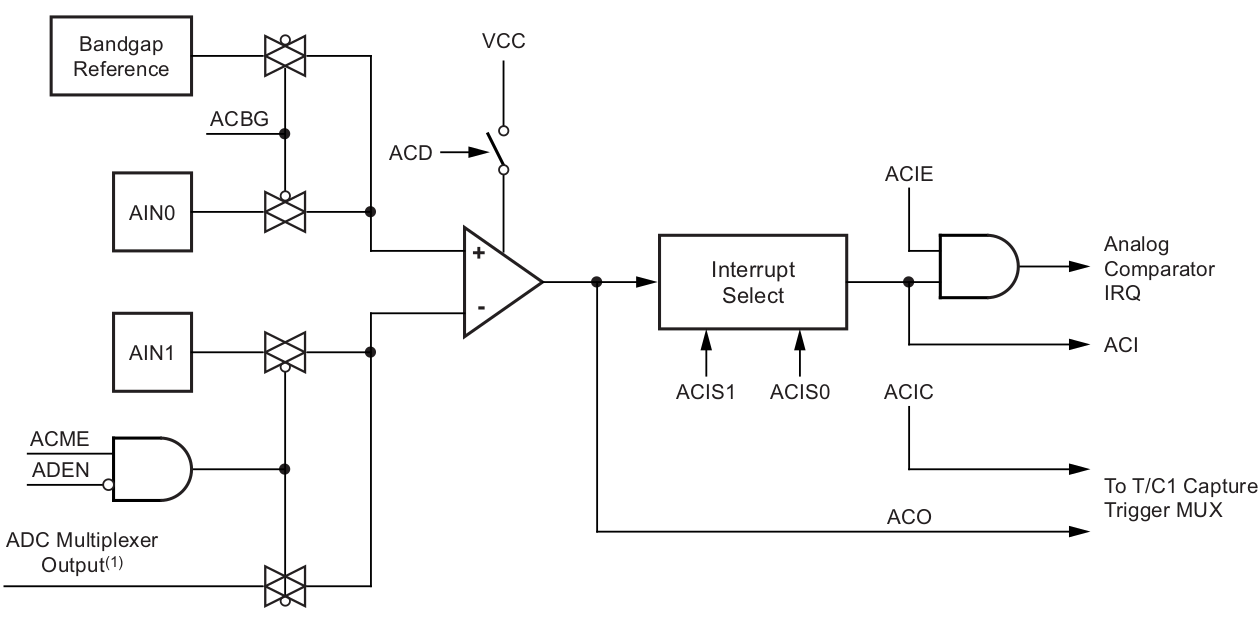
\includegraphics[width=1\textwidth]{AnalogComparatorBlock.png}
\end{figure}

\section{Analog Compartors Input}
\begin{itemize}
    \item One input is either be \pinFormat{AIN0} positive pin or Bandgap reference selected by \bitFormat{ACBG} bit.
    \item The other input can be either \pinFormat{AIN1} negative pin or any one of ADC multiplexed output selected by \bitFormat{ACME}, \bitFormat{ADEN} and \bitFormat{MUX[2:0]} pins.
\end{itemize}
\begin{table}[H]
    \centering
    \begin{tabular}{c|c|c|c}
        \bitFormat{ACME} & \bitFormat{ADEN} & \bitFormat{MUX[2:0]} & \textbf{Analog Compartor Negative Input}\\
        \hline
        0 & x & xxx & AIN1\\
        1 & 1 & xxx & AIN1\\
        1 & 0 & 000 & ADC0\\
        1 & 0 & 001 & ADC1\\
        1 & 0 & 010 & ADC2\\
        1 & 0 & 011 & ADC3\\
        1 & 0 & 100 & ADC4\\
        1 & 0 & 101 & ADC5\\
        1 & 0 & 110 & ADC6\\
        1 & 0 & 111 & ADC7\\
    \end{tabular}
\end{table}

\section{Register Description}
\subsubsection*{ADCSRB – ADC Control and Status Register B}
\vspace*{0.5cm}
\begin{bytefield}[bitformatting={\large\bfseries},
    endianness=big,bitwidth=0.125\linewidth]{8}
    \bitheader[lsb=0]{0-7} \\
    \bitbox{1}{\small -}
    \bitbox{1}{\small ACME}
    \bitbox{1}{\small -}
    \bitbox{1}{\small -}
    \bitbox{1}{\small -}
    \bitbox{1}{\small ADTS2}
    \bitbox{1}{\small ADTS1}
    \bitbox{1}{\small ADTS0}\\
\end{bytefield}

\subsubsection*{ACSR – Analog Comparator Control and Status Register}
\vspace*{0.5cm}
\begin{bytefield}[bitformatting={\large\bfseries},
    endianness=big,bitwidth=0.125\linewidth]{8}
    \bitheader[lsb=0]{0-7} \\
    \bitbox{1}{\small ACD}
    \bitbox{1}{\small ACBG}
    \bitbox{1}{\small ACO}
    \bitbox{1}{\small ACI}
    \bitbox{1}{\small ACIE}
    \bitbox{1}{\small ACIC}
    \bitbox{1}{\small ACIS1}
    \bitbox{1}{\small ACIS0}\\
\end{bytefield}

\begin{itemize}
    \item \bitFormat{ACD} - Analog Comparator Disable - The power to analog comparator is switched off when this bit is set to one.
    \item \bitFormat{ACBG} - Analog Comparator Bandgap Select - [1 - Selects Bandgap reference as positive input to analog comparator; 0 - Selects \pinFormat{AIN0} as positive input to analog comparator]
    \item \bitFormat{ACO} - Analog Comparator Output - The actual output of Analog Comparator.
    \item \bitFormat{ACI} - Analog Comparator interrupt Flag - Set by hardware when compartor output event triggers the interrupt mode.
    \item \bitFormat{ACIE} - Analog Comparator interrupt Enable - Enabled the analog comparator interrupt.
    \item \bitFormat{ACIC} - Analog Comparator Input Capture Enable - Enables the input capture function in Timer/Counter1 to be triggered by analog comparator.
\end{itemize}
\begin{table}[H]
    \begin{center}
        \begin{tabular}{c|c}
            \bitFormat{ACIS[1:0]} \textbf{- Analog Comparator Interrupt Mode Select} & \textbf{Interrupt Mode}\\
            \hline
            00 & Comparator interrupt on output toggle.\\
            01 & Reserved\\
            10 & Comparator interrupt on falling output edge.\\
            11 & Comparator interrupt on rising output edge.\\
        \end{tabular}
    \end{center}
\end{table}

\section{Configuring the Analog Comparator}
\subsection{Using AIN1 as positive input and AIN0 as Negative Input}
\begin{itemize}
    \item First, the Analog Comparator Multiplexer Enable bit (\bitFormat{ACME}) in \regFormat{ADCSRB} Register is diabled to select \pinFormat{AIN1} pin as positive input.
    \item Next, the Analog Comparator Bandgap Select bit (\bitFormat{ACBG}) in \regFormat{ADCSRB} Register is diabled to select \pinFormat{AIN} pin as negative input.
    \item Next, the interrupt mode is selected by Configuring the \bitFormat{ACIS[1:0]} bit in \regFormat{ADCSRB} register.
    \item The interupt for analog comparator is enabled by setting the \bitFormat{ACIE} bit in \regFormat{ADCSRB} register.
    \item Finally, the Analog Comparator is swithched on by clearing the \bitFormat{ACD} bit in \regFormat{ADCSRB} register.
    \item Also, the ISR is written for handling the interrupt.
    \item The code can be seen below:
\end{itemize}

\begin{minted}[breaklines, bgcolor=lightgray]{c}
// Disabling the Analog Comparator Multiplexer Enable bit so that AIN1 is selected as positive input
ADCSRB &= ~(1<<ACME);

// Disabling the Analog Comparator Bandgap Select bit so that AIN0 is selected as negative input
ACSR &= ~(1<<ACBG);

// Choosing the interrupt mode to toggle ACO bit 
// By selecting 00 to ACIS[1:0]
ACSR &= ~(1<<ACIS1);
ACSR &= ~(1<<ACIS0);

// Enabling the Analog Comparator interrupt Enable to see the output
ACSR |= (1<<ACIE);

// enabling the Analog Comparator by clearing the Analog Comparator Disable bit
ACSR &= ~(1<<ACD);
sei();

ISR(ANALOG_COMP_vect)
{
    PINC |= (1<<0);
}
\end{minted}
\end{document}
